\documentclass{article}
\usepackage{cmap}
\usepackage[utf8]{inputenc}
\usepackage[english,ukrainian]{babel}
\usepackage{graphicx}
\usepackage{geometry}
\usepackage{listings}
\usepackage{float}
\usepackage{amsmath}
\geometry{
	a4paper,
	left=20mm,
	right=20mm,
	top=15mm,
	bottom=15mm,
}
\lstset{
	language=c,
	tabsize=4,
	keepspaces,
	showstringspaces=false,
}
\graphicspath{ {./pictures} }
\setlength{\parindent}{4em}

\newcommand\subject{Основи електроніки}
\newcommand\lecturer{професор кафедри ПЗ \\ Фечан А.В.}
\newcommand\teacher{доцент кафедри ПЗ \\ Коцун В.І.}
\newcommand\mygroup{ПЗ-22}
\newcommand\lab{3}
\newcommand\theme{Аналіз перехідних процесів у колах із зосередженими
	параметрами засобами програмного продукту Multisim Live}
\newcommand\purpose{Навчитись аналізувати перехідні процеси у колах із зосередженими
	параметрами засобами програмного продукту Multisim Live}

\begin{document}
\begin{normalsize}
	\begin{titlepage}
		\thispagestyle{empty}
		\begin{center}
			\textbf{МІНІСТЕРСТВО ОСВІТИ І НАУКИ УКРАЇНИ\\
				НАЦІОНАЛЬНИЙ УНІВЕРСИТЕТ "ЛЬВІВСЬКА ПОЛІТЕХНІКА"}
		\end{center}
		\begin{flushright}
			\textbf{ІКНІ}\\
			Кафедра \textbf{ПЗ}
		\end{flushright}
		\vspace{200pt}
		\begin{center}
			\textbf{ЗВІТ}\\
			\vspace{10pt}
			до лабораторної роботи № \lab\\
			\textbf{на тему}: “\textit{\theme}”\\
			\textbf{з дисципліни}: “\subject”
		\end{center}
		\vspace{112pt}
		\begin{flushright}
			
			\textbf{Лектор}:\\
			\lecturer\\
			\vspace{28pt}
			\textbf{Виконав}:\\
			
			студент групи \mygroup\\
			Коваленко Д.М.\\
			\vspace{28pt}
			\textbf{Прийняв}:\\
			
			\teacher\\
			
			\vspace{28pt}
			«\rule{1cm}{0.15mm}» \rule{1.5cm}{0.15mm} 2023 р.\\
			$\sum$ = \rule{1cm}{0.15mm}……………\\
			
		\end{flushright}
		\vspace{\fill}
		\begin{center}
			\textbf{Львів — 2023}
		\end{center}
	\end{titlepage}
		
	\begin{description}
		\item[Тема.] \theme.
		\item[Мета.] \purpose.
	\end{description}

	\section*{Теоретичні відомості}

	
		\section*{Індивідуальне завдання}
	\begin{enumerate}
		\item Згідно отриманого завдання провести аналіз перехідних процесів в не
		розгалуженому колі змінного струму (для знаходження величин L та C
		прийняти за робочою частотою схеми 1кГц).
		\item Відтворити схему в середовищі Multisim Live та запустити її симуляцію.
		\item Побудувати часові залежності струмів та напруг схеми.
		\item Провести аналіз параметрів кола визначити тривалість перехідних
		процесів та максимальне відхилення струмів та напруг схеми в порівнянні
		з стаціонарними значеннями.
	\end{enumerate}
	
	\section*{Хід виконання}
	\begin{figure}[H]
		\centering
		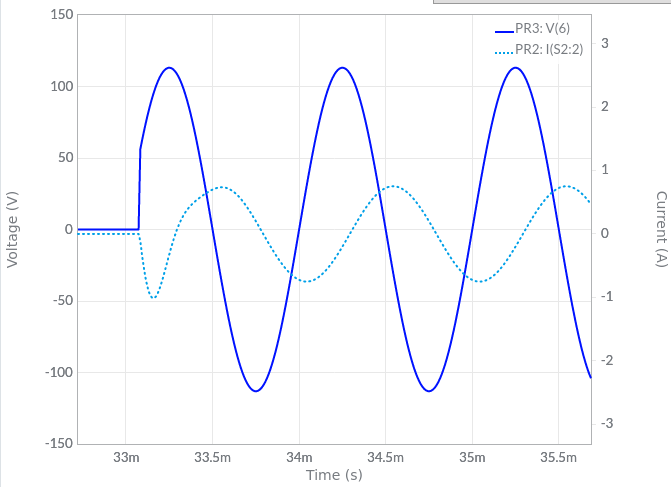
\includegraphics[scale=0.5]{11}
		\caption{Перехідний процес на резисторі.}
	\end{figure}
	
	\begin{figure}[H]
		\centering
		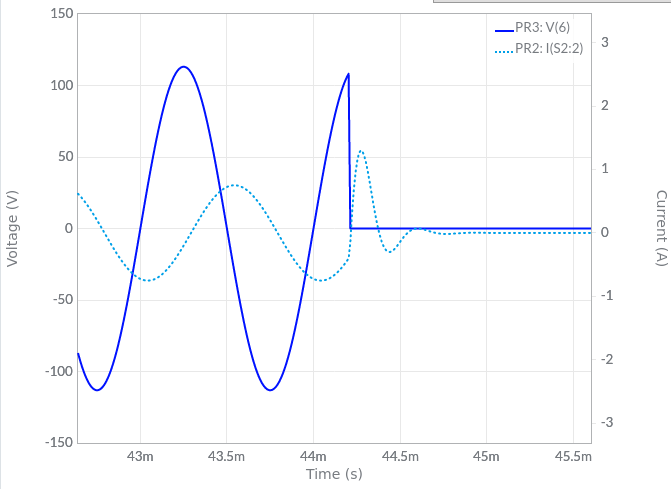
\includegraphics[scale=0.5]{12}
		\caption{Перехідний процес на резисторі.}
	\end{figure}

	\begin{figure}[H]
		\centering
		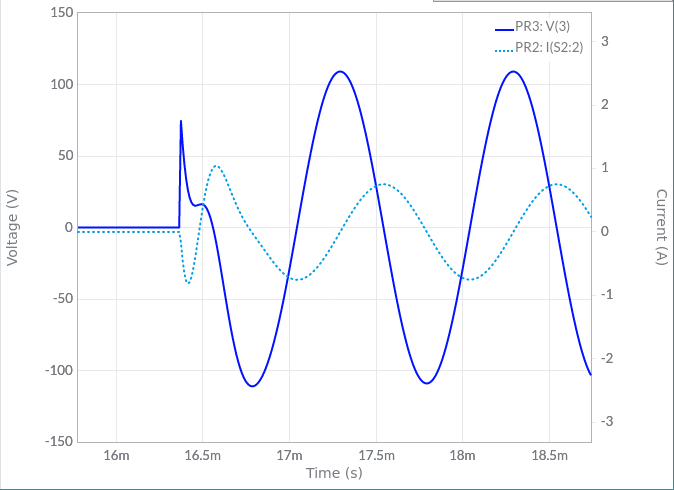
\includegraphics[scale=0.5]{21}
		\caption{Перехідний процес на котушці №1.}
	\end{figure}
	
	\begin{figure}[H]
		\centering
		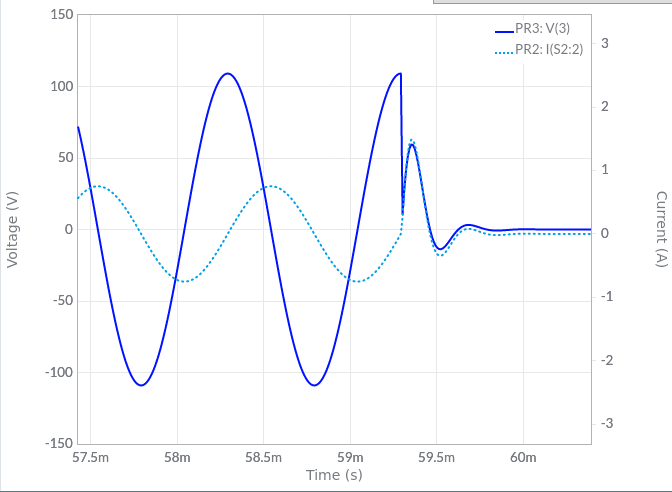
\includegraphics[scale=0.5]{22}
		\caption{Перехідний процес на котушці №1.}
	\end{figure}
	
	\begin{figure}[H]
		\centering
		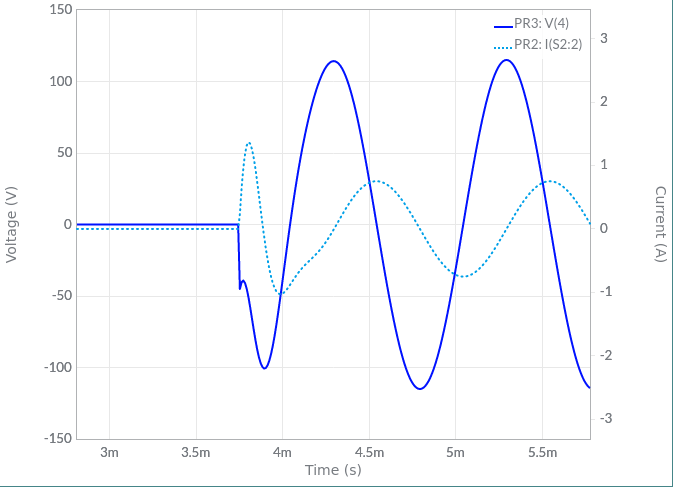
\includegraphics[scale=0.5]{31}
		\caption{Перехідний процес на котушці №2.}
	\end{figure}
	
	\begin{figure}[H]
		\centering
		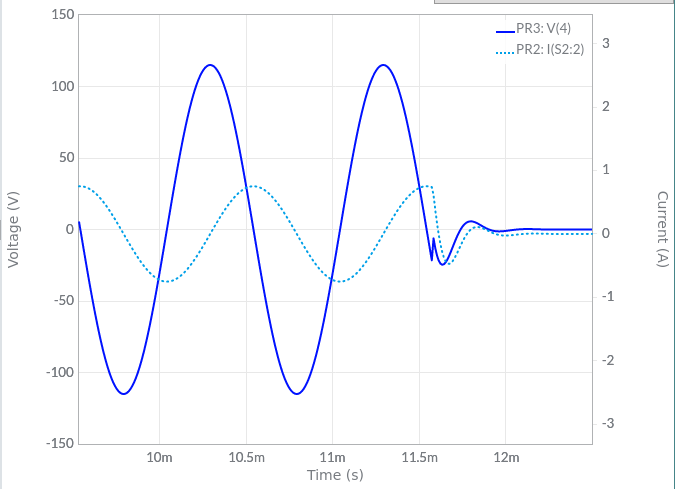
\includegraphics[scale=0.5]{32}
		\caption{Перехідний процес на котушці №2.}
	\end{figure}

	\begin{figure}[H]
		\centering
		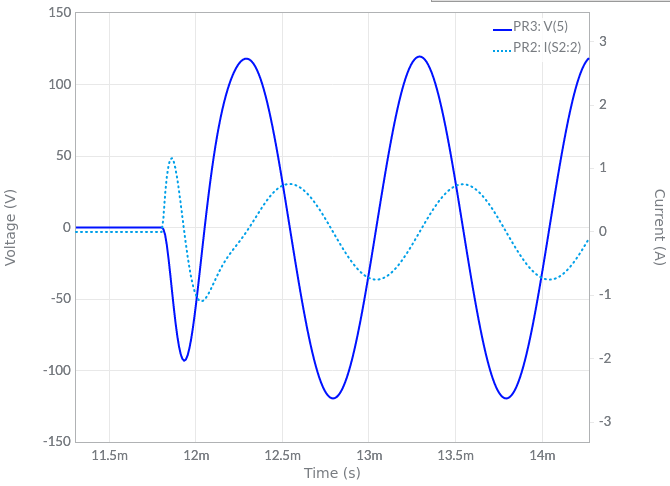
\includegraphics[scale=0.5]{41}
		\caption{Перехідний процес на конденсаторі.}
	\end{figure}
	
	\begin{figure}[H]
		\centering
		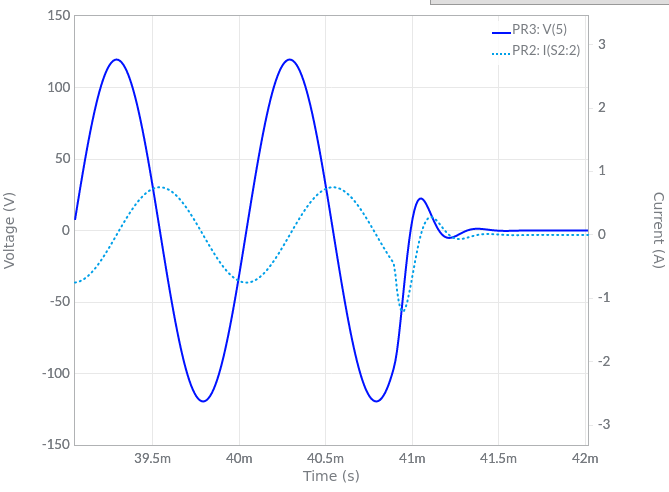
\includegraphics[scale=0.5]{42}
		\caption{Перехідний процес на конденсаторі.}
	\end{figure}

	\begin{table}[H]
		\centering
		\renewcommand*\arraystretch{1.3}
		\begin{tabular}{|p{0.15\linewidth}|p{0.2\linewidth}|p{0.2\linewidth}|}
			\hline
			& вимк. $\rightarrow$ увімк., мс & увімк. $\rightarrow$ вимк., мс \\
			\hline
			Резистор & 0.5 & 0.5 \\
			\hline
			Котушка №1 & 0.5 & 0.7 \\
			\hline
			Котушка №2 & 0.5 & 0.6 \\
			\hline
			Конденсатор & 0.4 & 0.6 \\
			\hline
		\end{tabular}
		\caption{Часові залежності струмів та напруг схеми.}
	\end{table}

	\section*{Висновки}
	Під час виконання лабораторної роботи я навчився аналізувати перехідні процеси у колах із зосередженими параметрами засобами програмного продукту Multisim Live.
	    
\end{normalsize}
\end{document}
